\documentclass[a4paper, 12pt]{article}

% Íslenskan jaaá
\usepackage[icelandic]{babel}
\usepackage[T1]{fontenc}

% Pakkar

\usepackage{amsmath, amssymb, amsthm}

\usepackage{titlesec}
\usepackage{calc}
\usepackage{url}

\usepackage[hang,flushmargin]{footmisc}
\usepackage{tabularx}
\usepackage{enumitem}
\usepackage{booktabs}
\usepackage{hyperref}
\usepackage{tcolorbox}
\usepackage{listings}
\usepackage{listingsutf8}
\usepackage{xcolor}
\usepackage{colortbl}

\definecolor{codegreen}{rgb}{0,0.6,0}
\definecolor{codegray}{rgb}{0.5,0.5,0.5}
\definecolor{codepurple}{rgb}{0.58,0,0.82}
\definecolor{backcolour}{rgb}{0.95,0.95,0.92}

\lstdefinestyle{mystyle}{
    backgroundcolor=\color{backcolour},   
    commentstyle=\color{codegreen},
    keywordstyle=\color{magenta},
    numberstyle=\tiny\color{codegray},
    stringstyle=\color{codepurple},
    basicstyle=\ttfamily\small,
    breakatwhitespace=false,         
    breaklines=true,                 
    captionpos=b,                    
    keepspaces=true,                 
    numbers=left,                    
    numbersep=5pt,                  
    showspaces=false,                
    showstringspaces=false,
    showtabs=false,                  
    tabsize=2
}

\lstset{style=mystyle}

\usepackage{pgfplots}
\pgfplotsset{compat=1.17}

\usepackage{times, mathptmx}
\usepackage[scaled=0.85]{beramono}
\usepackage{seqsplit} % til að splitta löngum texttt umhverfum

\newcommand{\doctitle}{\uppercase{HEIMADÆMI 2}}
\newcommand{\coursename}{Tölvunarfræði 2}
\newcommand{\coursenum}{TÖL203G}

% Stærðfræðitákn
\renewcommand{\qedsymbol}{$\blacksquare$}

% ——— Mengjatákn
\newcommand{\N}{\mathbb{N}}
\newcommand{\Z}{\mathbb{Z}}
\newcommand{\Q}{\mathbb{Q}}
\newcommand{\R}{\mathbb{R}}
\newcommand{\C}{\mathbb{C}}

% ——— Vigrar
\renewcommand{\u}{\mathbf{u}}
\renewcommand{\v}{\mathbf{v}}
\renewcommand{\b}{\mathbf{b}}
\newcommand{\w}{\mathbf{w}}
\newcommand{\p}{\mathbf{p}}
\newcommand{\x}{\mathbf{x}}
\newcommand{\y}{\mathbf{y}}
\newcommand{\z}{\mathbf{z}}


\begin{document}
\vspace*{.5cm}
\centerline{\bfseries\Large\doctitle}
\medskip
\centerline{\large\coursenum\ \coursename}
\bigskip
\bigskip
\centerline{\large Kári Hlynsson}
\bigskip
\centerline{Háskóli Íslands}
\medskip
\centerline{Vormisseri 2023}
\bigskip
\bigskip

\large

\noindent
\textbf{Verkefni 1.} \\
Biðröð (\emph{queue}) sem er útfærð með fylki sem hefur tvo vísa (\emph{indexes}): \texttt{head}
og \texttt{tail} (sjá glæru 13 í fyrirlestri 3).

\begin{enumerate}[label=(\alph*)]
  \item Hver geta gildin á þessum tveimur vísum verið þegar biðröðin er tóm? Rökstyðjið í nokkrum orðum.
  \item Hver geta gildin á þessum tveimur vísum verið þegar biðröðin er full? Rökstyðjið í nokkrum orðum.
\end{enumerate}

\noindent
\textbf{Lausn.} Látum $Q$ tákna biðröðina sem um ræðir.

\begin{enumerate}[label=(\alph*)]
  \item Þegar $Q$ er tóm vísa $\texttt{head}$ og $\texttt{tail}$ á sama stað í fylkinu. Ef við bætum hlut við á $Q$ færist $\texttt{last}$ áfram um eitt skref í fylkinu.

  \item Þegar $Q$ er full vísa $\texttt{head}$ og $\texttt{tail}$ á sama stakið í fylkinu. Því könnum við alltaf hvort \texttt{head} = \texttt{tail} (eða hliðstæð útfærsla í þeirri
  gagnagrind sem er notuð) þegar við ætlum að bæta nýju staki við en ef svo er þurfum við að kalla á \texttt{Resize()} aðgerðina til að stækka fylkið.
\end{enumerate}

\newpage

\noindent
\textbf{Verkefni 2.} \\
Bókin er með útfærslu á biðröð með fylki af breytilegri lengd: \texttt{\seqsplit{ResizingArrayQueue.java}}. Í henni er aðferðin \texttt{Resize} sem er notuð til að stækka/minnka
fylkið þegar þörf er á. Búið til sýnidæmi þar sem þið byrjið með biðröðina á æfingunni á glæru 14 í fyrirlestri 3. Hún inniheldur 4 stök og er í fylki af stærðinni (\emph{capacity})
6.

\begin{enumerate}[label=(\alph*)]
  \item Setjið tvö stök inn í þessa biðröð og sýnið stöðuna á henni eftir það.
  \item Setjið svo eitt stak í viðbót (sjöunda stakið) inn í biðröðina og sýnið hvernig fylkið lítur út eftir
    að \texttt{Resize} aðferðin sem gefin er í bókinni hefur verið framkvæmd.
\end{enumerate}

\noindent
\textbf{Lausn.} Við samtvinnum liðina saman.
Fyrir neðan sjáum við töfluna í upphafsstöðu.
\setlength{\tabcolsep}{15pt}
\renewcommand{\arraystretch}{1.25}
\begin{table}[ht!]
  \centering
  \begin{tabular}{lcccccc}
    \toprule
    \texttt{q[]} &  \texttt D &  \textit{null} &  \textit{null} &  \texttt A &  \texttt B &  \texttt C \\
                 & \texttt 0 & \texttt 1             & \texttt 2             & \texttt 3 & \texttt 4 & \texttt 5 \\
    \bottomrule
                 &  & \texttt{tail} & & \texttt{head} & & \\
  \end{tabular}
\end{table}

\noindent
Bætum nú stökunum \texttt E og \texttt F við, en þá lítur biðröðin svona út:
\begin{table}[ht!]
  \centering
  \begin{tabular}{lcccccc}
    \toprule
    \texttt{q[]} &  \texttt D &  \texttt E &  \texttt F &  \texttt A &  \texttt B &  \texttt C \\
                 & \texttt 0 & \texttt 1             & \texttt 2             & \texttt 3 & \texttt 4 & \texttt 5 \\
    \bottomrule
                 &  &  &  & \texttt{head} & & \\
                 &  &  &  & \texttt{tail} & & \\
  \end{tabular}
\end{table}

\noindent
Ef við reynum nú að bæta við \texttt G í biðröðina er kallað á \texttt{Resize()} og stærð nýju biðraðarinnar verður tvöföld
hinnar fyrri, í þessu tilfelli 12. Þá lítur biðröðin einhvern veginn svona út:

\newpage
\begin{table}[ht!]
  \centering
  \begin{tabular}{lcccccccccc}
    \toprule
    \texttt{q[]} & \texttt A & \texttt B & \texttt C &  \texttt D &  \texttt E &  \texttt F & \texttt G & \textit{null} & \ldots \\
                 & \texttt 0 & \texttt 1 & \texttt 2 &  \texttt 3 &  \texttt 4 &  \texttt 5 & \texttt 6 & \texttt 7 & \ldots \\
    \bottomrule
                 & \texttt{head} &  &  & & & & & \texttt{tail }\\
  \end{tabular}
\end{table}

\noindent
Þess er ekki þörf að skrifa út restina af biðröðinni, vegna þess að rest stakanna eru \textit{null} og innihalda því litlar
upplýsingar. (Að auki kæmist taflan ekki fyrir á síðunni :-|)

\newpage
\noindent
\textbf{Verkefni 3.} \\
Gefið slöngutáknun fyrir eftirfarandi föll:
\begin{enumerate}[label=(\alph*)]
  \item $f(N) = N \sqrt N + \frac{N^3 + N^2 \log N}{N}$
  \item $f(N) = 3(N + 1)^3 + 2N^2 \log N$
  \item $f(N) = \frac{\log N^3 + 1}{\log N^2} + \frac 1N$
\end{enumerate}

\noindent
\textbf{Lausn.}
\begin{enumerate}[label=(\alph*)]
  \item Athugum að
  \[
    f(N) = N \sqrt N + \frac{N^3 + N^2 \log N}{N} = N \sqrt N + N^2 + N \log N
  \]
  Af þessum föllum er $N^2$ stærsti vaxtarflokkurinn svo slöngutáknunin er $f(N) \sim N^2$.

  \item Sviginn $3(N + 1)^3$ gefur þriðja stigs margliðu í $N$ með stuðulinn $3$ framan við $N^3$.
    Af þeim liðum sem koma fyrir er $N^3$ mest afgerandi svo $f(N) \sim 3N^3$.

  \item Reiknireglur logra gefa
   \[
     f(N) = \frac{\log N^3 + 1}{\log N^2} + \frac 1N = \frac{3 \log N + 1}{2 \log N} + \frac 1N = \frac 32 + \frac{1}{2 \log N} + \frac 1N
   \]
  Báðir seinni liðanna stefna á núll þegar $N \to \infty$ svo ráðandi liðurinn hér er fastinn $\frac 32$, þ.e. $f(N) \sim \frac 32$.
\end{enumerate}

\newpage
\noindent
\textbf{Verkefni 4.} \\
Finnið vaxtarhraða á keyrslutíma sem fall af $N$ fyrir forritsbútinn í æfingadæminu hér að ofan. Sýnið vaxtarhraðann með slöngutáknun og rökstyðjið
svar ykkar með útreikningum.

\medskip
\noindent
\textbf{Lausn.} Við viljum gefa upp kostnaðarlíkan forritsbútsins fyrir neðan m.t.t. inntaksstærðar. Veljum hækkun á \texttt{sum} breytunni sem fulltrúa
í greiningunni. 

\begin{lstlisting}[language=java]
 long sum = 0;
  for (long i=1; i<=N; i=2*i)
    for (long j=1; j<=2*i; j++)
        sum++; 
\end{lstlisting}

\noindent
Í hverri ítrun tvöfaldar ytri \texttt{for} lykkjan
gildið á \texttt i svo við getum ætlað að hún keyri $\lg N$ sinnum.

Innri for lykkjan ítrar yfir bilið $\{1, \ldots, 2N\}$ (í raun ítrar hún yfir allar hlutrunanna
$\{1, \ldots, 2i\}$ með $1 \leq i \leq N$, en vægi þeirra er lítið í samhengi við síðasta liðinn, þar
sem $i \approx N$). Aðgerðin \texttt{sum++} tekur fastan tíma. Við getum nú tekið þetta saman og fáum
að kostnaðarlíkanið okkar er
\[
T(N) = \lg N \cdot 2N \cdot 1 \sim N \lg N
\]
Við skulum útfæra notendaforritið \texttt{TimeFunc.java} sem notar \texttt{Stopwatch} klasann úr algs4 kóðasafninu til að bera saman kostnaðarlíkanið
við hermd gildi. Klasinn er á næstu síðu.

Fyrstu tímamælingar aðrar en $0.0$ fara ekki að koma fram fyrr en $N = 536870912$ svo taflan byrjar auðvitað þar. Tafla 1 á bls. 7 sýnir mælingarnar
auk tvöföldunarhlutfalls fyrir $T(N)$ út frá mældu gildunum en Mynd 1 sýnir tvöföldunarhlutfallið sem fall af $N$. Athugum að $T(2N)/T(N)$ sem ber saman
við kenningu okkar um að forritsbúturinn hafi tímaflækju $T(N) \sim N \lg N$.

\newpage
\begin{lstlisting}[language=java]

  import edu.princeton.cs.algs4.Stopwatch;

  public class TimeFunc {
  
    /**
     * The function we want to obtain an amortized
     * cost model for.
     *
     * @param N size of input
     * @return evaluation of sum for given N
     */
    public static long sum(long N) {
      long sum = 0; 
      for (long i=1; i<=N; i=2*i)
        for (long j=1; j<=2*i; j++) 
          sum++;
      return sum;
    }
  
    /**
     * Times the sum function.
     *
     * @param N input size to run N with
     * @return runtime in seconds
     * @see Stopwatch
     */
    public static double timeTrial(long N) {
      Stopwatch timer = new Stopwatch();
      long ignore = sum(N);
      return timer.elapsedTime();
    }
    
    public static void main(String[] args) {
      for (long N = 1; N <= Long.MAX_VALUE; N = 2*N) 
        System.out.printf("%12d\t%7.1f\n", N, timeTrial(N));
    }

  }
  
\end{lstlisting}

\newpage

\begin{table}[ht!]
  \centering
  \caption{Tímamælingar hermana með inntakstærð $N$}
  \begin{tabular}{lcr}
    \toprule
    N              & Tími (s)  & $T(2N)/T(N)$ \\
    \midrule
    \ldots         & \ldots & \ldots \\
    536870912	     & 0.1  & — \\ 
    1073741824	   & 0.8  & 8.00 \\
    2147483648	   & 2.9  & 3.62 \\
    4294967296	   & 5.8  & 2.00 \\
    8589934592	   & 11.5 & 1.98 \\
    17179869184	   & 24.0 & 2.09 \\
    34359738368	   & 48.5 & 2.02 \\
    68719476736	   & 95.8 & 1.98\\
    137438953472	 & 187.1 & 1.95 \\
    \bottomrule
  \end{tabular}
\end{table}

\begin{figure}[ht!]
  \centering
  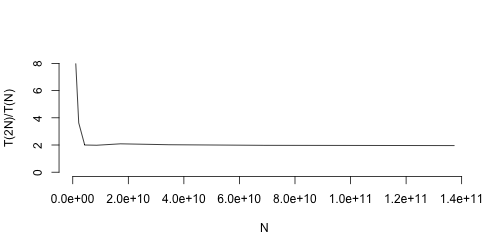
\includegraphics[width=\textwidth]{rplot.png}
  \caption{Hlutfallið $T(2N)/T(N)$ sem fall af $N$}
\end{figure}

\newpage

\noindent
\textbf{Verkefni 5.} \\
Í þessu dæmi eigið þið að fylla inn í töflu þar sem línurnar eru stærð
inntaks og dálkarnir vaxtarhraði á keyrslutíma (tímaflækja) nokkurra reiknirita, gefinn með slöngutáknun.
Hvert sæti töflunnar á að innihalda tímann sem tiltekið reiknirit myndi taka á þessari inntaksstærð, miðað
við tölvu þar sem hver aðgerð tekur 1 nsek. ($1 \cdot 10^{-9}$ sek.). Til að koma ykkur af stað er búið að
fylla inn í eitt hólfið. Þetta þurfa ekki að vera nákvæm gildi (t.d. 1 klst. í stað 3536.28 sek.).

\medskip
\noindent
\textbf{Lausn.} Taflan er fyrir neðan. 

\begin{table}[ht!]
  \begin{tabular}{l|c|c|c|c}
    \toprule
                  & $\sim 4 \lg N$ & $\sim 10 N \lg N$ & $\sim 2N^2$ & $\sim \frac{1}{10} 2^N$ \\
    \midrule
    $N = 10$      & 13.3 ns        & 0.33 µs           & 0.20 µs         & 0.10 µs                 \\
    $N = 10^2$    & 26.6 ns        & 6.64 µs           & 20 µs           & 1.27e+20 s                 \\
    $N = 10^3$    & 39.9 ns        & 1.00 ms           & 20 ms           & 1.07e+291 s                       \\
    $N = 10^6$    & 79.8 ns        & 0.20 s            & 33 mín.         & Óendanlegt                        \\
    $N = 10^9$    & 0.12 µs        & 5 mín.            & 63 ár        & Óendanlegt                       \\
    \bottomrule
  \end{tabular}
\end{table}

\end{document}
